\chapter{Application and System Implementation}
\label{ch:application}

All screenshots in this chapter were captured on 17 November 2026 by an automated Playwright script (\code{report/scripts/capture\_screenshots.mjs}) driving the application while it was connected to the real checkpoints. A fresh, separate database was used, and all messages are controlled examples written for this purpose. Nothing was mocked or edited after capture apart from cropping.

\section{Application architecture}
The application is a local web application: a FastAPI service (\cref{ch:architecture}) and a React single-page application served from the same process. The interface follows the layout of a team chat client. A sidebar lists the channel (\emph{\#team-chat}), the Dependencies, Timeline and Model results pages, the settings and a ``viewing as'' switch. Since the application has no login, this switch lets a demonstrator act as each participant in turn (Riya, project lead; Anushree, data engineer; Bianca, ML engineer). The main view has the channel on the left and a tasks panel on the right with three sections: \emph{Needs you} (suggestions the current person may decide), the person's tasks or the whole team's, and a collapsed \emph{Waiting on teammates} section.

Messages are entered either in \emph{Live AI} mode, typed in the composer and analysed by the models, or replayed from one of six scripted \emph{demo stories}. In demo stories the extraction is pre-written and labelled \code{scripted}, while reconciliation, review, history and the graph are the real code. Scenario F, written for this report's demonstration, has 17 messages that exercise every operation and every kind of dependency the system recognises.

\section{Task management workflow}
\Cref{fig:shotneeds} shows the workspace during Scenario F, viewed as Riya after she has asked Bianca to share a results report. The two suggestions derived from that message, the new task and its dependency on the evaluation script, appear under \emph{Waiting on teammates}: only Bianca can accept them. Riya can dismiss them, because she wrote the message, and can switch to Bianca's view. Under each message a chip summarises what the system made of it (``2 accepted'', ``2 suggestions to review'').

\begin{figure}[t]
\centering
\shot{01_workspace_needs_you}
\caption[Workspace during a demo story]{Workspace during Scenario F, viewed as Riya. The suggestions from her latest message wait for Bianca, the person they affect. The demo player at the bottom shows who speaks next.}
\label{fig:shotneeds}
\end{figure}

\subsection{Approval, rejection and modification}
\Cref{fig:lifecycle} summarises the mechanisms. A suggestion can be:
\begin{itemize}
  \item \textbf{accepted} by an affected person, after the safety checks of \cref{sec:reconciliation}; the change is applied and history events are appended;
  \item \textbf{edited and accepted}, through a dialog that starts from the suggested values (title, owner, due date, or which task a reference means); edited fields are recorded with source kind \code{human};
  \item \textbf{dismissed} by an affected person or by the author of the message; nothing changes except the suggestion's status;
  \item \textbf{taken or left open}, for a new task with no identifiable owner: the viewer can take it, leave it unassigned for a volunteer, or assign it explicitly through the edit dialog.
\end{itemize}
Accepted tasks can still be modified directly in a task sheet (title, owner, status, due date). These edits are version-checked: an edit based on an outdated version is refused.

\begin{figure}[t]
\centering
\diagram{lifecycle}
\caption[Task lifecycle and safety]{Proposal and task lifecycle. A pending proposal is applied only if the reviewer is an affected person and the safety checks pass; otherwise nothing is written. Stored task states follow the allowed transitions, and the graph derives ready, blocked and needs-review states from them.}
\label{fig:lifecycle}
\end{figure}

\subsection{Task modification proposals}
\Cref{fig:shotdate} shows the two-step date change. Bianca asked to move her evaluation-script deadline to Friday, and that request was accepted as a proposal. In the team list the task still shows its original due date (Thursday 12 November), with the pending move marked ``New date Fri 13 Nov awaiting OK''. Riya has replied ``Friday is fine.'', which the reconciler recognised as a confirmation of the pending proposal; it now waits under Riya's \emph{Needs you}. Only when Riya accepts it does the due date change.

\begin{figure}[t]
\centering
\shot{02_date_change_confirmation}
\caption[A task modification proposal]{Two-step date change. The pending move is shown on the task but not applied; Riya's short reply has become a confirmation that only she may accept.}
\label{fig:shotdate}
\end{figure}

\section{Successful extraction in Live mode}
\Cref{fig:shotlive} shows four messages analysed by the real models, viewed as Bianca. Riya's \emph{``Bianca please prepare the quarterly report by Friday.''} produced a card titled ``Prepare the quarterly report'', due Friday 13 November, assigned to Bianca, with the question raised by the deadline/scheduled conflict (\cref{sec:walkthrough}). The team-wide \emph{``Please book the demo meeting for next Tuesday.''} names nobody, so the system does not invent an owner: it asks which person should book the meeting and offers \emph{I'll take it} and \emph{Leave open}. The chat also shows how non-actionable messages are treated. \emph{``The server went down yesterday.''} produced no proposal at all, and \emph{``Thanks, that sounds good!''} was recognised as an acknowledgement with no pending change.

\begin{figure}[t]
\centering
\shot{06_live_extraction}
\caption[Live extraction with the real models]{Live mode with the real checkpoints and the hybrid preset, viewed as Bianca: a named request with owner and deadline, an unassigned team request, and two non-actionable messages.}
\label{fig:shotlive}
\end{figure}

\section{Explaining a suggestion: the AI Inspector}
Every message has a ``How AI read this'' panel. \Cref{fig:shotinspector} shows it for the quarterly-report message. Panel (a) shows the refined spans with their origins and the rule that changed them; panel (b) switches to the raw neural spans, where the fragmentation is visible. Further tabs show links with scores, the resolution of dates and owners, the reconciler's decision with matching scores and flags, and the sources of every stage (\cref{fig:shotsources}, left), including the pipeline configuration and model versions.

\begin{figure}[t]
\centering
\begin{subfigure}[t]{0.49\linewidth}\centering
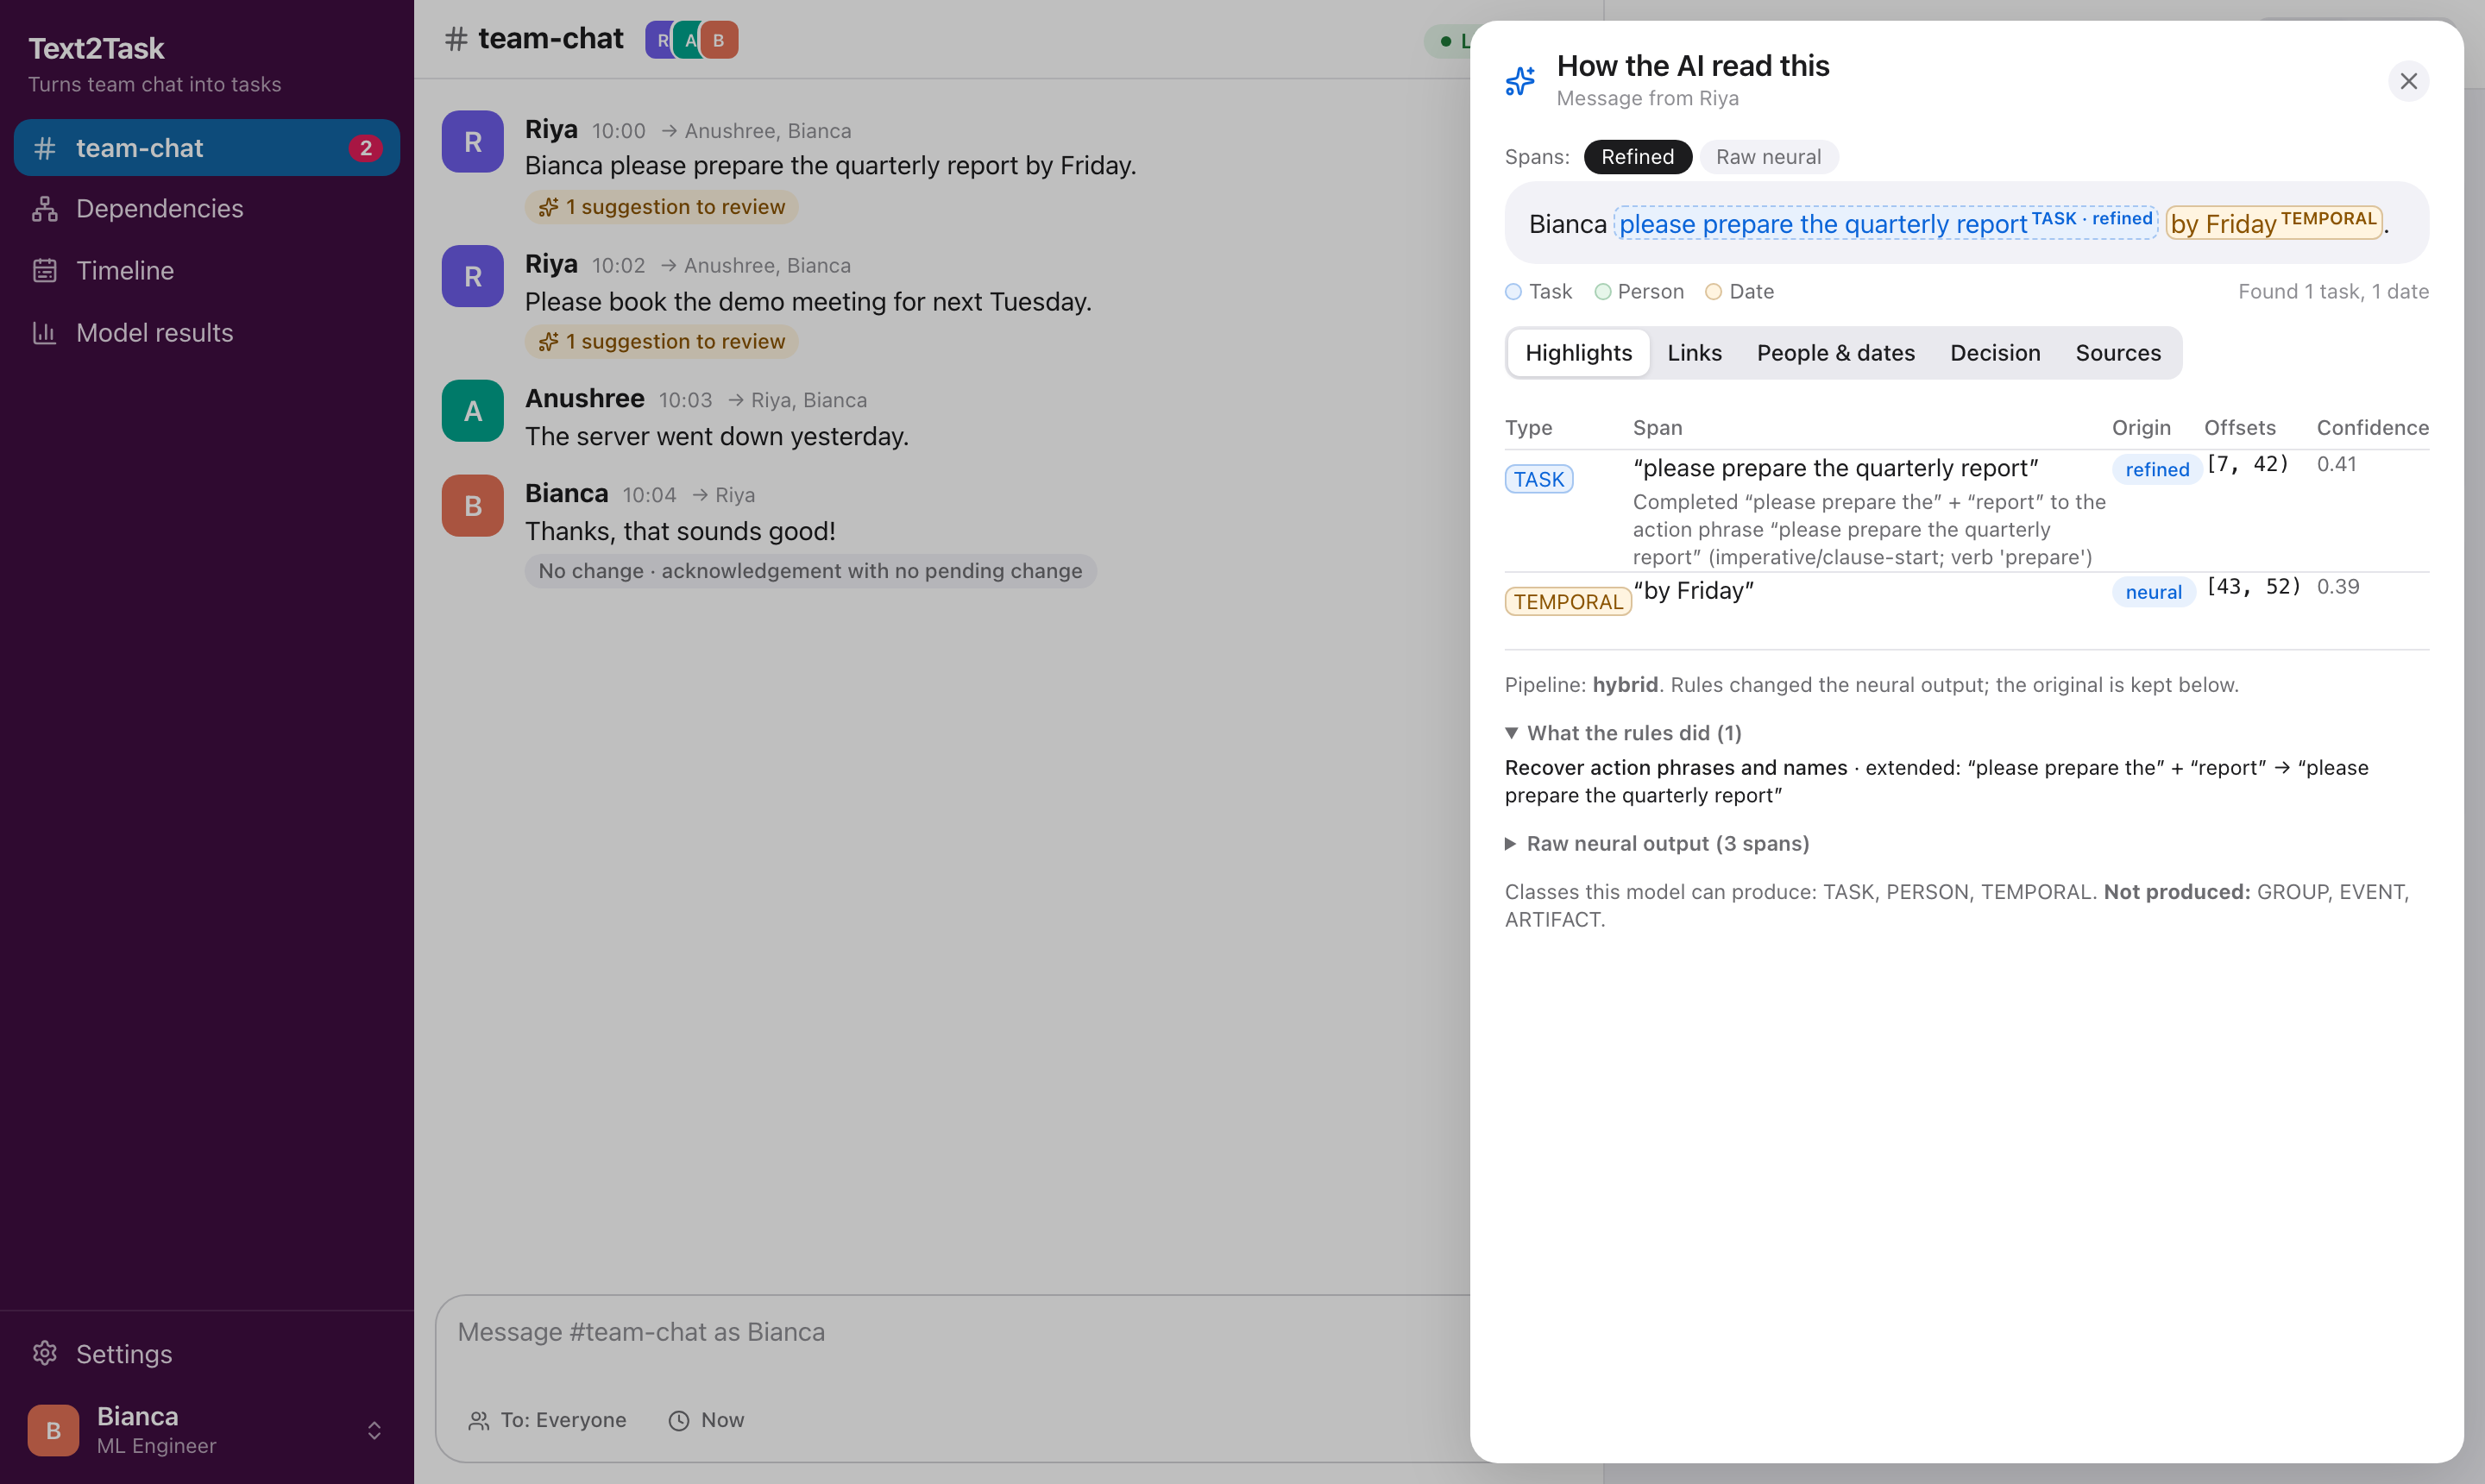
\includegraphics[width=\linewidth, trim=1690 330 20 0, clip]{figures/screenshots/07_inspector_hybrid.png}
\caption{Refined spans (hybrid)}\end{subfigure}\hfill
\begin{subfigure}[t]{0.49\linewidth}\centering
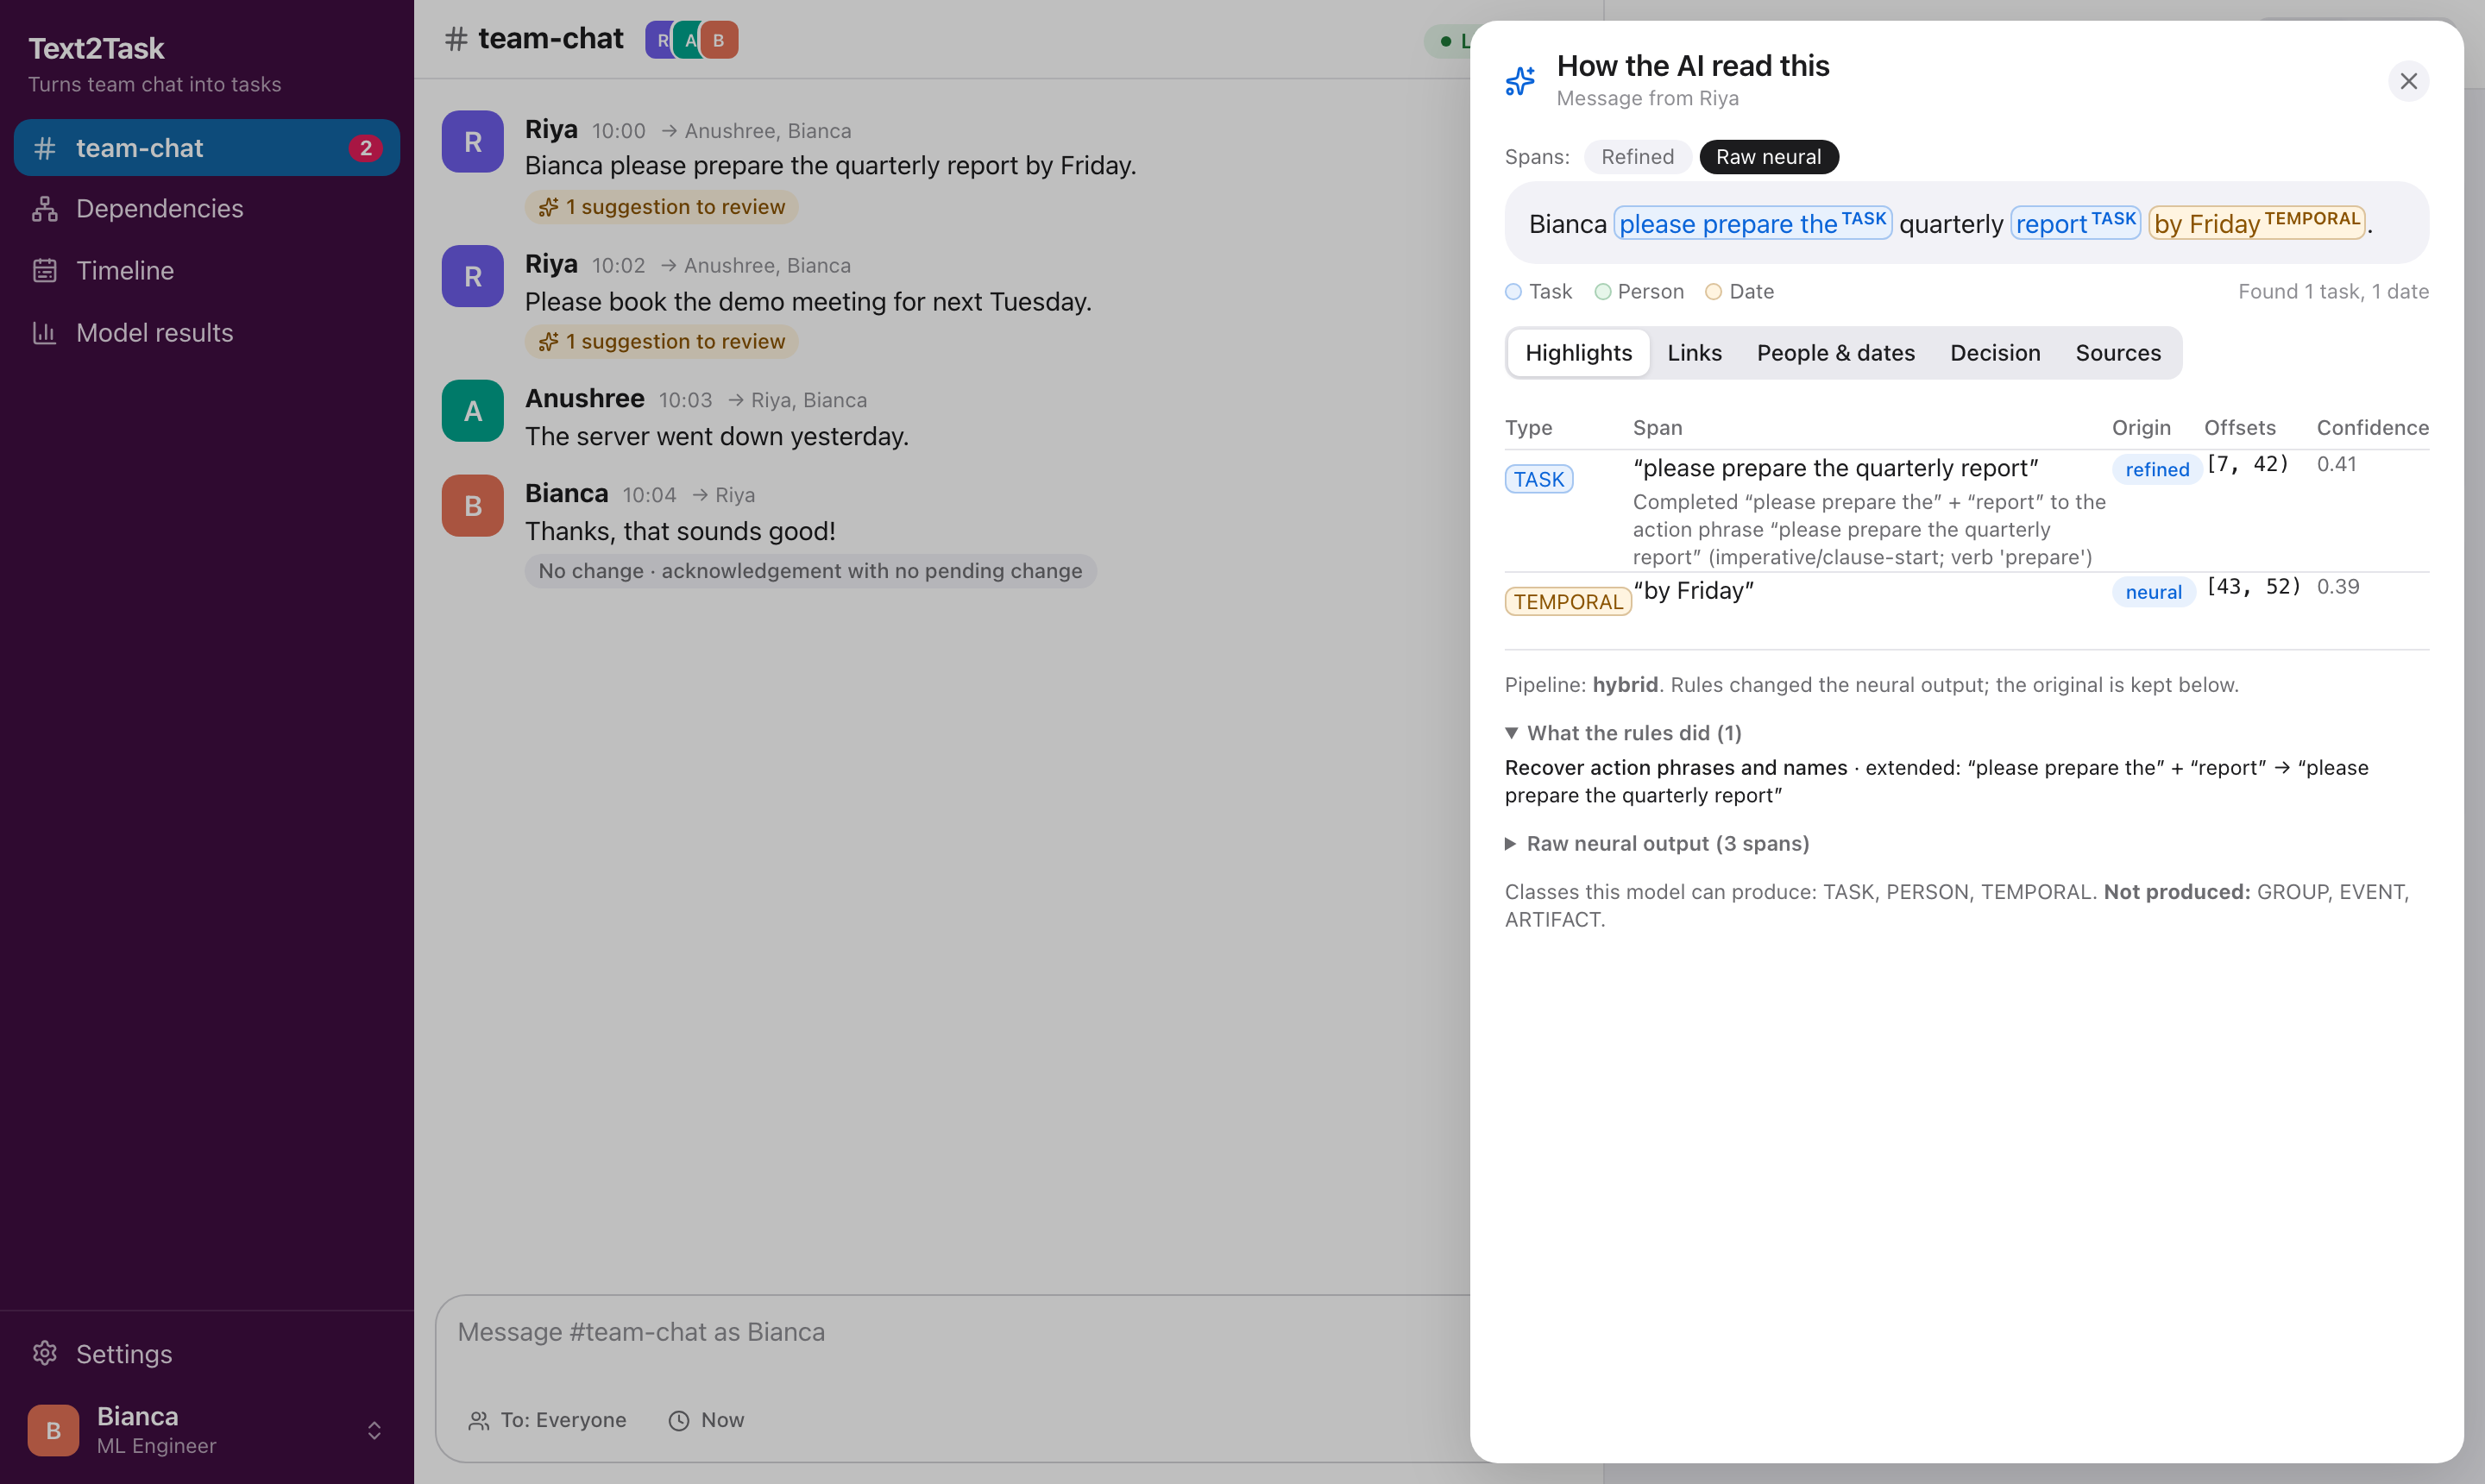
\includegraphics[width=\linewidth, trim=1690 330 20 0, clip]{figures/screenshots/08_inspector_raw_neural.png}
\caption{Raw neural spans}\end{subfigure}
\caption[AI Inspector: refined versus raw spans]{The AI Inspector for the worked example. The raw entity model produced two TASK fragments and missed \emph{quarterly}; grammar recovery joined them into one refined span and records what it did.}
\label{fig:shotinspector}
\end{figure}

\section{Ambiguous requests}
\Cref{fig:shotamb} shows Scenario C. Two open, unowned tasks exist, ``review the slides'' and ``review the slides for the client deck''. When Anushree writes \emph{``I can review the slides.''}, the sentence matches both. The card asks which task she means, and the edit dialog lists both candidates with their match scores. Nothing changes until she picks one.

\begin{figure}[t]
\centering
\shot{05_ambiguous_referent}
\caption[Ambiguous reference]{An ambiguous reference (Scenario C). The volunteer's sentence matches two tasks; the dialog shows both candidates and changes nothing until a person chooses.}
\label{fig:shotamb}
\end{figure}

\section{A failure case}
\Cref{fig:shotsources} (right) shows a known failure, documented in the Phase 7.5 report and reproduced here. For \emph{``Bianca, call me after the meeting.''} the clause-dependency stage reads \emph{after} as a prerequisite cue and the neural model marks \emph{the meeting} as a TASK, so the analysis contains two TASK spans (\emph{call me} and \emph{the meeting}) and a dependency between them, where a person would see one request with a time reference. In the same session \emph{``Deployment can't start until the test server is set up.''} produced no dependency, because the reconciler's lexical matcher found no existing tasks to attach it to. Both are discussed in \cref{ch:errors}.

\begin{figure}[t]
\centering
\begin{subfigure}[t]{0.49\linewidth}\centering
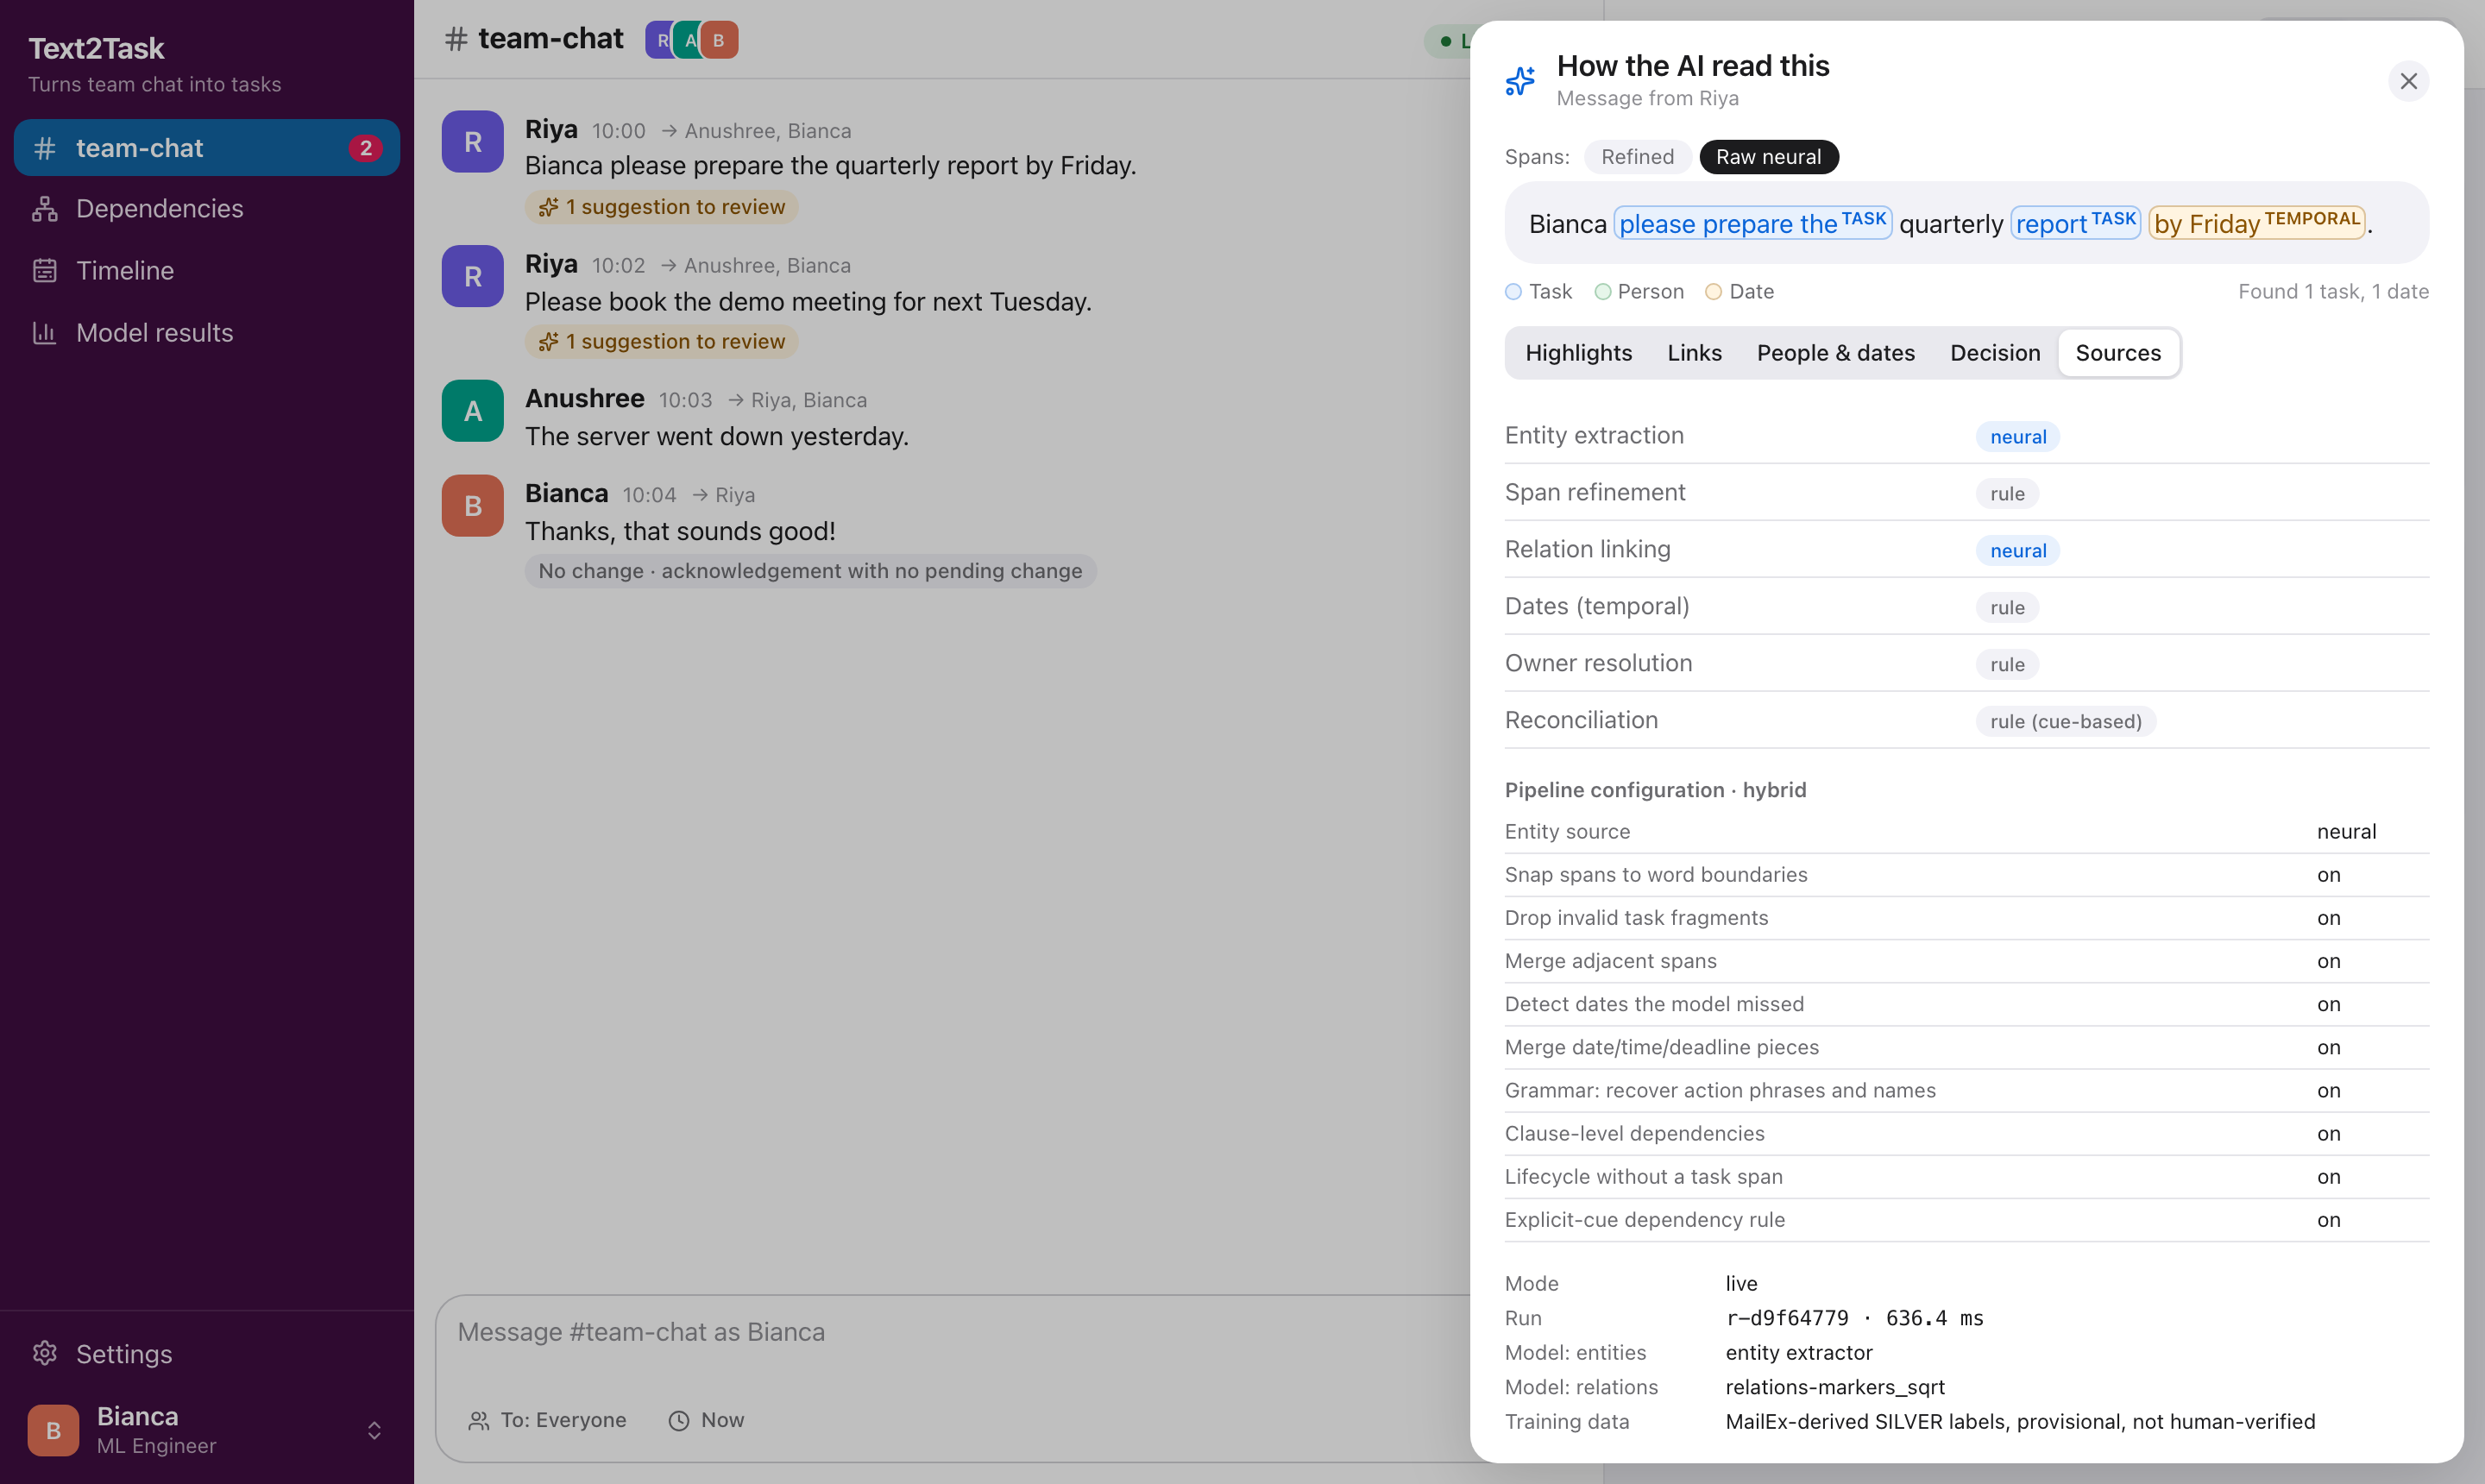
\includegraphics[width=\linewidth, trim=1690 0 20 0, clip]{figures/screenshots/09_inspector_sources.png}
\caption{Sources and pipeline configuration}\end{subfigure}\hfill
\begin{subfigure}[t]{0.49\linewidth}\centering
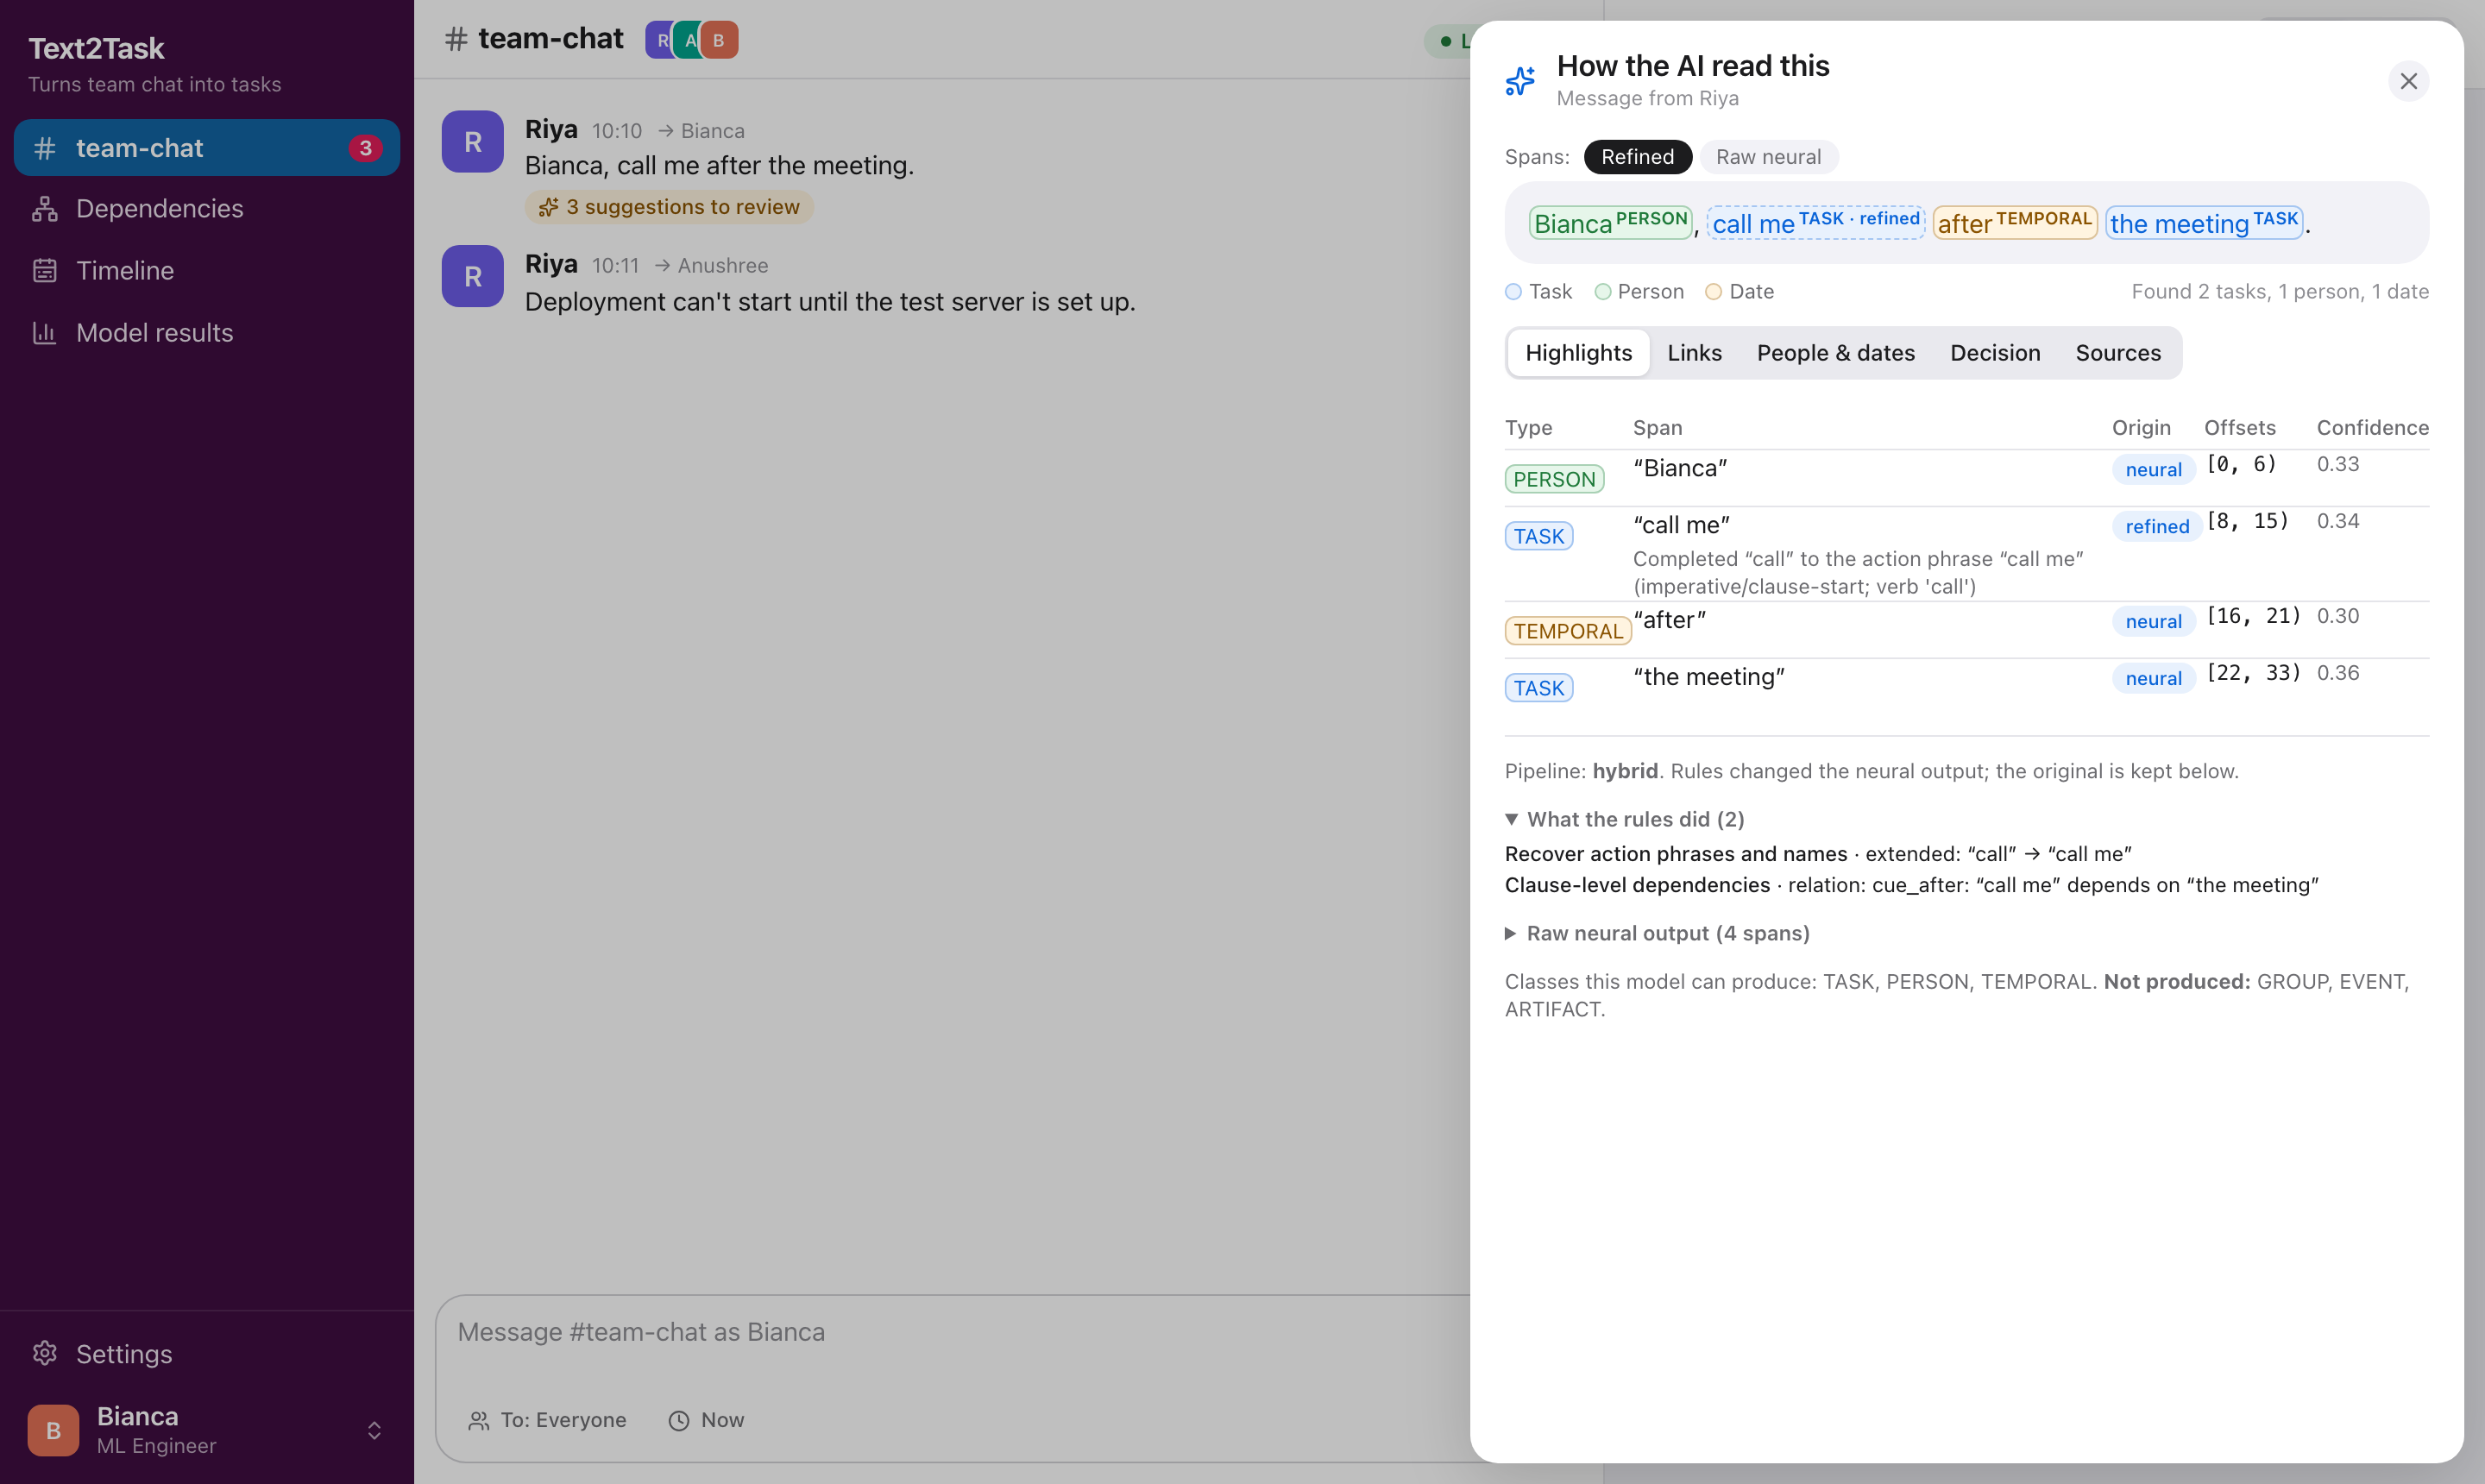
\includegraphics[width=\linewidth, trim=1690 0 20 0, clip]{figures/screenshots/10_failure_case.png}
\caption{False positive: ``call me after the meeting''}\end{subfigure}
\caption[Inspector sources tab and a failure case]{(a) The Sources tab lists which component produced each part of the analysis, the refinement switches, the run time and the model versions, and states that the training labels are not human-verified. (b) A failure: \emph{the meeting} is treated as a task and \emph{after} as a dependency cue.}
\label{fig:shotsources}
\end{figure}

\section{Dependencies and timeline}
\Cref{fig:shotgraph} shows the dependency explorer at the end of Scenario F. The graph contains a chain (collect reviews $\to$ clean dataset $\to$ train model $\to$ build dashboard), a fan-in (the dashboard waits on training, the demo server and the evaluation script), a fan-out (the evaluation script blocks two tasks), a held edge drawn as a red dotted line because it would have closed a cycle, and a task in \emph{needs review} because its only prerequisite was cancelled. The side panel shows the selected task and a what-if preview. \Cref{fig:shottimeline} shows the timeline: one row per person, one column per day, with deadlines and planned dates distinguished and undated tasks listed rather than placed on a guessed day.

\begin{figure}[t]
\centering
\shot{03_dependency_graph}
\caption[Dependency explorer]{Dependency explorer at the end of Scenario F, with every kind of dependency the system recognises, a held cycle-forming edge and a task flagged for review after its prerequisite was cancelled.}
\label{fig:shotgraph}
\end{figure}

\begin{figure}[t]
\centering
\shot{04_timeline}
\caption[Timeline]{Timeline view: open tasks placed on their confirmed due (flag) or planned date, by person; tasks without a confirmed date appear under ``No date yet''.}
\label{fig:shottimeline}
\end{figure}

\section{Backend execution}
\Cref{lst:serverlog} is an excerpt of the server log from the screenshot session, and \cref{lst:caps} is the capability report the interface reads to decide whether Live mode is available. Both are copied verbatim (ports removed).

\lstinputlisting[style=terminal, caption={Server log excerpt from the screenshot session (\code{figures/screenshots/terminal\_server\_log.txt}).}, label={lst:serverlog}]{figures/screenshots/terminal_server_log.txt}

\lstinputlisting[language=json, caption={Capability report returned by \code{/api/system/capabilities} during the session (selected fields).}, label={lst:caps}]{figures/screenshots/terminal_capabilities.json}

\section{Testing of the application}
The application is covered by 362 backend unit and API tests (including reviewer-rights, scenario and refinement tests), 97 frontend component tests with automated accessibility checks, and 20 Playwright end-to-end tests, of which 13 run against a scripted-only server and 7 against a server with the real models. The end-to-end suite also guards earlier defects, for example a styling regression that made selected buttons illegible, and the reviewer rule (``the project lead cannot accept a task assigned to Anushree'').
